\documentclass{article}
\usepackage[margin=0.5in]{geometry}

\usepackage{listings}
\usepackage{enumitem}
\usepackage{appendix}
\usepackage{graphicx}


\title{ESE532 Project Final Report - Group}
\author{Ritika Gupta, Taylor Nelms, and Nishanth Shyamkumar}

\begin{document}

\maketitle

\section{Introduction}
The elephant in the room for the entirety of our implementation is that, as of 24 hours before the due date of this project, it is not functioning correctly.
It gets through the entirely of the input, and (finally) does not hang in the middle of a deadlock or infinite loop somewhere in hardware, but upon encoding and decoding some files (particuarly, long binary files), the decoded version does not match the original.
\newline\newline
Now, that does not mean we cannot obtain reasonable ideas as to performance, area/time costs, etc. for our design. However, concerns such as specific design axes eluded us through development because we were unable to reach the essential milestone of "a working design."
\newline\newline
This is all to say that, while we cannot empirically verify any results of design changes, or give good accounts of verification strategies, what we \textbf{can} do is evaluate design decisions we could have made through the process, and analyze what kind of effects they would have on a mythical end result where our software worked.
\newline\newline
As such, you must excuse us if we are light on some empiric details, as we, even in this final stretch, endeavor to improve our design to the point of functionality. 90-minute build times are, unfortunately, not condusive to rapid prototyping, so we will do what we can to represent our control of the source material in an academic sense, if not always a practical one.

\section{Single ARM processor design}

\subsection{Performance achieved and Energy required:}
The throughput performance achieved for an all software design, i.e, where each of the algorithms were running on the Arm core was 7Mbps. 
\newline\newline 
The energy required for this design was 
Power = 2.22W 
\newline
Time = 40 minutes = 2400 seconds
\newline
Energy = PT = 2.22 * 2400 
\newline
       = 5328 Joules

\subsection{Compression achieved: }
    Input file : vmlinuz.tar       
    \newline
    Input size : 66MB
    \newline
    Compressed size: 36.6MB
    \newline\newline

\subsection{Time spent on major components:}

Rabin : 286011cycles
\newline
        Throughput : 59Mbps
\newline\newline
Sha : 407923 cycles
\newline
      Throughput : 41.53Mbps
\newline\newline
LZW : 1023284 cycles
\newline
Throughput : 16.56Mbps
\newline


\section{Ultra 96 design}
– Performance achieved and energy required
– Compression achieved
– Key design aspects: task decomposition, parallelism, mapping to Zynq resources, include diagrams to support
– Be clear where each component of the final design is performed (e.g., ARM, NEON vector, FPGA logic).
– Model to explain performance, area, and energy of design
– Current bottleneck preventing higher performance

All the components CDC, SHA, LZW and deduplication operate in hardware. 
Input data is read from network and it is processed in 2MB parts. 


\subsection{Compression achieved:}

    Input file : LittlePrince.txt       
    \newline
    Input size : 14KB
    \newline
    Compressed size: 4.4KB
    \newline\newline
    
    Input file : ESE532.tar       
    \newline
    Input size : 50KB
    \newline
    Compressed size: 24.2KB
    \newline\newline

    Input file : Franklin.txt       
    \newline
    Input size : 390KB
    \newline
    Compressed size: 308KB
    \newline\newline

    Input file : vmlinuz.tar       
    \newline
    Input size : 66MB
    \newline
    Compressed size: 36.6MB
    \newline\newline

    Input file : linux.tar       
    \newline
    Input size : 191MB
    \newline
    Compressed size: 60.9MB
    \newline\newline


\subsection{Processor components:}

Input data is read from network and it is processed in 2MB parts. 
\newline
The input read over the network is handled using a pthread that is executing on its own core. 
\newline
The primary processor core(core 0) is running the PS section that interfaces with the PL logic. 
\newline
The network thread is bound to run only on core 2. 
\newline

\subsubsection{Network thread functionality} 

The thread uses a 200MB input buffer that is shared between the cores 2 and 0.
\newline
The NW thread then reads packets, calculates the length of each packet and then copies over the bytes to the buffer.
\newline
In our implementation, we use 2MB buffers to feed the dataflow model implemented on the FPGA.
\newline
So the NW thread has the additional responsibility to increment a counter everytime it crosses the 2MB boundary. 
This variable is checked against in the main processor to make certain that it does not try to process any data before the buffer data fills up. The variable is used as a synchronization mechanism.
\newline
Finally upon exit, the NW thread indicates that it has completed its purpose and marks a variable that is used by core 0 to figure out that no more packets are to be expected.
\newline

\subsubsection{Output thread functionality}

There is a 3rd thread outside of the main and network thread that is tasked with writing processed data onto a file. 
\par
The output thread is bound to core 3 and it is responsible for opening, closing files and of course writing the data to the file. 
It is invoked based on the existing synchronization mechanisms and it frees the processor 0 from having to deal with write backs to the file. 
\newline

CDC performs chunking and the data is taken by SHA and LZW which operate parallely. The output of SHA which is 256 bit SHA value and the compressed output of LZW are both taken by deduplicate section to finally write the appropriate output to the output file. 
3 ARM cores are being used. One is used for reading the input data, one for processing the data and the third for writing the output to the output file.  

\subsection{FPGA Design}

%TODO: put our awesome diagram of our data flow

\subsubsection{Hardware Wrapper}

On the outside of our PL functionality, we have a wrapper function that allows us to have a singular top-level function that operates on a larger buffer than a single chunk, but a smaller amount of data than an entire file.
\par
For us, this has meant calling an overall function on a $2{MB}$ section of data. This was chosen to be larger than a single chunk by a few factors of scale, while being small enough to allow for sensible passing of data into the PL.
\newline\par
This wrapper function, \texttt{processBuffer}, sets up the relevant streams between components and calls each of those component functions. 
Each component is responsible for reading and writing from its relevant stream for as many times as it needs across the entire length of that input buffer.
\par
It contains simple functions for turning the internal streams into the whole-buffer sizes that SDx likes, which allows us to use a \texttt{SEQUENTIAL} access pattern on our data as a whole. That way, each interface, effectively, is implemented as a FIFO.
\newline\par
Each of the streams internally are $9$-bit value streams; that way, we could allow for delimiting 'bytes', which marked the ends of chunks or the end of the buffer overall (represented internally as \texttt{ENDOFCHUNK} and \texttt{ENDOFFILE} macros).
\par
The one exception to this was the output from the \texttt{SHA} unit, as its output was always a set of $32$ 8-bit values matched to the number of chunks coming out of \texttt{LZW}.

\subsubsection{Rabin Fingerprinting}

\subsubsection{SHA-256}

\subsubsection{LZW}

Given that the algorithm for compression itself involves, conceptually, one memory lookup, one memory write, and one read from the input stream for each incoming byte,
a streaming and pipelined approach seemed most appropriate.
\par
As it stands, we implement this operation using a small hash table and simplistic hash function which uses as its 'key'
the conceptual address of the 'large-memory' LZW-table implementation (which would require 8k rows of $256$ columns each, each of which would contain a $13$-bit value).
\par
For this, we elected to hash this key down to 10 bits, using an arbitrary (but relatively effective) hash function to cut down on computational requirements.
This meant we had $1024$ hash rows, and we elected to allow for $24$ entries into each; a factor of $8$ was used to allow for the potential $8k$ table rows, and an extra factor of $3$ was to allow for hash collisions and similar overflows.
\par
A more careful implementation would allow for a small associative memory to handle such overflow; however, given the time constraints, we did not do this.
\newline\par
The one last consideration we had was the burden of 'resetting' the table for each chunk.
Writing all of the values to our chosen 'Not Found' value (\texttt{0x1FFF}) would be a huge memory strain.
\par
As such, we elected to have another table of validity bits, to mark which parts of the LZW hash table were valid for that iteration.
This would require only $1024$ 24-bit values, which were easier to reset for each chunk than the entire hash table.

\subsubsection{Deduplication}

This function includes the calls to the \texttt{chunkDict} location of shared memory, containing the records of each \texttt{SHA} digest and its matching index.
\newline\par
Given the potentially large number of output chunks, we could not keep these records in the PL memory. 
As such, we implemented a rough dictionary in shared memory, hashing the digest down to $16$ bits with a simple \texttt{XOR} strategy,
and using that to index into our shared memory area.
\par
We decided to allow for some degree of hash collisions here; with a potential worst-case of roughly $2^{17}$ chunks to store digests for,
we allowed a factor-of-2 safety on our hash function, leading to $4$ records per hash bucket. 
There's a reasonable chance that this decision
is leading to our woes of things not working; a larger stretch of time would have allowed for better analysis on this point.

\par
The rest of the function was pedestrian by comparison; it reads the entire \texttt{LZW} stream (so no excess data is left) into a buffer,
as well as the entire incoming \texttt{SHA} digest that corresponds to it.
\par
Depending on whether or not there was a match in our dictionary, the relevant header is made for the output chunk,
and either just that header, or the entire LZW-compressed section, is sent to the output stream.


\subsection{Bottleneck}

Thanks to our decision to leverage the \texttt{DATAFLOW} pragma to handle our data movement in the PL, we have exactly zero idea of what the bottleneck in our design is.
\par
I know, that's not a great answer. When we try to make traces of our program execution, no tools that xilinx provides us allow for any kind of per-element trace of execution, or logs of streams being full/empty, or any other kind of relevant information. The best we have to go on are estimates of latencies of our functions, but, given that some of them run across variable-length chunks a variable number of times within our hardware buffer, the ranges are huge, and not reflective of actual execution.
\newline\par
However, what we \textbf{can} do is make estimates of what the bottlenecks might be. For instance: with a hardware buffer a couple factors of scale past our largest chunk workload, we can estimate that the data movement to and from the FPGA is not the primary concern; that overhead should amortize out far past any dominating bottleneck term.
\newline\par
So where, in our core logic inside the PL, could the bottleneck be? It is possible that it is the compute within the \texttt{SHA} function; there are certainly a lot of loops to perform for each block of $512$ bytes, and that necessarily takes time.
\par
Alternatively, the \texttt{LZW} unit could be the bottleneck. Though the inner function, which operates on a per-chunk basis, has been pipelined down to an \texttt{II} of $6$ (at 200MHz) or $9$ (at 300MHz), the overhead of clearing the validity bits for its hash table could be styming its ability to efficiently handle data at a high throughput.
\par
Our current bottleneck suspect is the access to shared memory for looking at the dictionary of \texttt{SHA} digests; this necessarily stalls the \texttt{deduplicate} unit until it can read a (current) total of $144$ bytes from shared memory for each chunk, which it then compares against our incoming \texttt{SHA} value. Depending on how efficiently this operation can work, this may hang up the entire operation. It is also possible that having to wait for this to be done before beginning to output our constructed packet to our final output stream could be holding back the design.
\par
The rest of our operations should be safe from bottlenecks; the reading of hardware buffer input into streams, the output from the final stream, and the process of Rabin-fingerprinting have all been pipelined effectively to initiation intervals of less than or equal to $2$.
\newline\par
Obviously, there are a lot of potential culprits, but the current front-runners are likely the \texttt{SHA} unit and the lookup section of the \texttt{Deduplicate} unit.

\section{10 Gbps design}

As has been noted, the fact that we are operating on a \texttt{DATAFLOW} model means that our ability to peek inside the specifics of our design is limited. Xilinx does not like putting that many (read: any) calipers on the internals of our hardware function.
\par
As such, we must examine possibilities for improvements in the abstract. In this section, we will discuss strategies for improving performance which, were we to work as diligently across the next $5$ weeks as we have for this previous $5$, would certainly yield performance improvements in pursuit of a $10Gbps$ goal.

\subsection{With Hardware Bounds in Mind}

Looking at our current design, we can approach designing a \texttt{10Gbps} design with the idea that the core functionality would still use logic almost entirely on the FPGA, but we could use more of our resources to solve the problem, and use as many tricks as possible to maximise the utility of the PL's time.
\newline\par
One of the first things we can see from our current resource usage is that we have a good number of BRAM's still available, as well as a large proportion of our FF/LUT resources.
This opens us up to putting more SHA units (for the computational resources) and LZW units (for the memory resources) onto the PL, with the idea that one of the two (likely the former) is the bottleneck culprit.
\par
With the idea that a singular \texttt{deduplicate} unit would still need to control output, we could link the \texttt{rabin} unit to the \texttt{deduplicate} unit by way of multiple parallel \texttt{SHA} units; for this example, we will imagine $2$ such units. This would allow us to alternate which unit hashed which series of chunks, allowing for an idealized $2x$ speedup on that axis.
\par
As for the \texttt{LZW} unit, we could easily fit another onto the PL in the same fashion.
\newline\par
If the resources are not the bottleneck, then we would need to look into the process by which we are transferring data. the use of \texttt{hls::stream} FIFO units has been handy for automatically handling a lot of timing requirements, but they carry the disadvantage of limiting the rate by which we are (conceptually) pipelining data through our application.
\par
One way we could improve upon this would be to use multiple streams in parallel for our application; conceptually, this would be similar to, instead of sending water through a single garden hose, sending water through two parallel garden hoses.
\par
If our bottleneck in the PL is access to the shared memory inside which our SHA dictionary resides, we could mitigate that problem by decreasing the amount of memory we need to read. We could do this by expanding our shared memory hash table region; if we're expecting something along the lines of $2^{16}$ unique chunks in a file, we could allocate $2^{19}$, or more, total hash lines such that we would probabilistically only need to pull one hash line for any given SHA digest.
\par
In this way, our total memory access would be in the range of $36$ bytes per chunk, rather than our current $144$. The disadvantage would be, we may need a particularly significant field of hash values to near-guarantee that we would not encounter any hash collisions that may break our design.
\newline\par
On our software side, we are currently using one thread/core purely to read in input, one to write to our output memory, and then one thread is copying memory to the FPGA working region, invoking the PL function, and then copying that memory out to a location from which the final thread writes.
\newline\par
A different implementation would more cleverly synchronize the operations that the middle thread performs, and make sure that the relevant memory copying did not need to happen (or at least, did not need to happen in a redundant fashion.)

\subsection{With No Hardware Bounds in Mind}

If we distance ourselves from the bounds of the Ultra96 system, however, we can consider all manner of other design options.
\par
Let us approach this by keeping the core of our design (the use of streaming data, the \texttt{DATAFLOW} pragma, and doing \texttt{LZW} and \texttt{SHA} in parallel), and seeing what additional resources could add to our design.
\newline\par
One thing that could immediately help our design would be to have a fully-associative memory for the records of what the \texttt{SHA} digest was for each chunk index. Putting such a memory into small, local memories would allow for extremely fast lookups in service of deduplication.
\par
By removing the need for shared memory access, that bottleneck could be completely eliminated. Further, it would only take a roughly 5MB memory to do so.
\newline\par
Considering our PL resources, if \texttt{SHA} is the bottleneck, the operation could be distributed across a huge number of computational units. In a similar fashion, given that each chunk is independent from the perspective of the \texttt{LZW} functionality, as many hardware units as possible could be thrown at that problem.
\par
Going further, and expanding on the idea of parallel streams, any issues of transferring the data across FIFO units could be distributed to allow for, 
for instance, the \texttt{Rabin} computation or \texttt{Deduplication} units to pipeline data through at a quicker speed than would be otherwise possible, 
writing a larger number of bytes per FPGA "cycle" and further reduce the effective \texttt{II} of our \texttt{DATAFLOW}-pipelined design.
\newline\par
On the software side, we wouldn't anticipate needing sweeping structural changes. Instead, we would benefit from those cores being slightly faster. At \texttt{10Gbps}, a new byte is coming in roughly every cycle for a \texttt{1.2GHz} processor. 
With a \texttt{2.4GHz} core, along with similarly-increased memory access capabilities, we could better assure that we did not drop packets somewhere in the process of moving all that data around.
\par 
As tempting as it would be to throw more threads at the task of reading input in, we fear that the overhead of synchronizing all such resources would outstrip the benefit of more processors doing the work.
\par
That said, a dedicated data mover and hardware buffer to handle the incoming data could allow for the best and safest resource handling at \texttt{10Gbps}.

\section{Validation techniques}
As of now the main validation technique is to run a script that can decode the compress.dat file generated from the application and then compares it with the input file that was sent over the network. 

We also use prints on the main arm core, that prints the bytes read by the network thread, to provide real time testing validation that all bytes are being read and no packets are being dropped. 
\section{Key lessons learned}

\section{Design space exploration}

\section{Key lessons learned}
\begin{description}
  \item[$\bullet$ ] It is always good to define the interfaces first and make a working implementation first and then incrementally add functionalities so that we always have something to fall back to ans start with a working code again.
  \item[$\bullet$ ] We learned how to make decisions when there is a memory-time trade off as there are limited memory and processing resources on the FPGA. 
  \item[$\bullet$ ] We learned to use many more optimization techniques by using various pragmas to decrease the time it takes to run and also the memory it takes. 

\end{description}

\section{Design space exploration}

Describe design space explored and show graphs and models to support design selection
For our earlier implementation in which we were running only LZW in hardware, the data was being sent to hardware for LZW and then the output back to the processor region to do the next steps in the computation, which led to very low speed of the overall implementation because of this data transfer overhead and most of the part still running in software. 
\newline
But that incremental way of putting things in hardware helped us ultimately moving the entire design to the hardware. So, now all the components CDC, SHA, LZW and deduplication all run in hardware. This removed the delay of transferring intermediate results between the FPGA and the processor region and also increased the overall speed because of hardware acceleration techniques like using pipelining, unrolling, partitioning arrays etc.
\newline\newline
To make advantage of running in hardware. we used dataflow pragma and serialized everything so that as soon as the data is available, the hardware component can start processing on it. 
\newline
CDC provides chunk data to SHA and LZW simultaneously, which operate in parallel. The flow of our design is described in Figure 1.
\newline\newline

\begin{figure}[h!]
  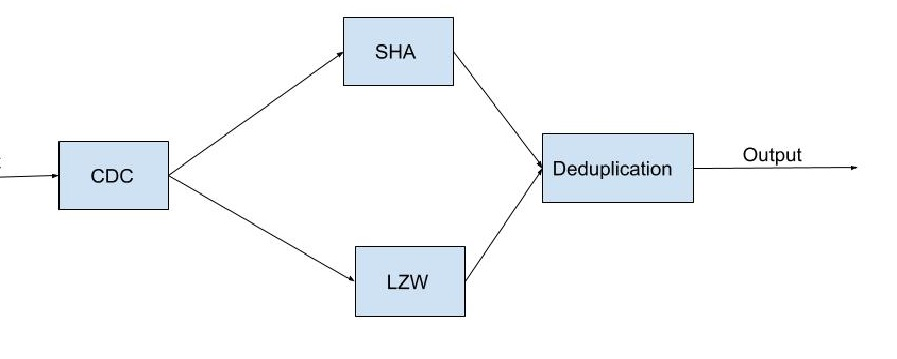
\includegraphics[width=\linewidth]{data_flow.jpg}
  \caption{Data flow.}
  \label{fig:data_flow}
\end{figure}

To save space on FPGA memory, we use shared memory to store our hash table for the deduplication step.
Another optimization technique was to use separate arm cores to read the input data from ethernet, to process on the data and to write the data to the output file. 
\newline
That saves time in the sense that it doesn't have to wait for the data transmission to complete before it can start processing on the data already read. So, one core reads the data from the ethernet and writes it to the shared memory, another core reads it and transfers it to the FPGA as soon as 2MB data has been written to it, and the third core writes the output data as soon as the 2MB data has been processed in the FPGA. This makes the overall implementation faster. 
\newline\newline\newline

The changes in what speed we get while moving from all software to all hardware is shown in the following table:
\begin{center}
\begin{tabular}{ |c|c|c|c|c| } 
 \hline
 \textbf{Implementation}  & \textbf{All Software} & \textbf{LZW in hardware} & \textbf{All hardware} & \textbf{All hardware with dataflow} \\ 
 \hline
 \textbf{Speed}           & 7 Mbps      & 15 Mbps    & 10 Mbps      & 193 Mbps \\ 
 \hline
\end{tabular}
\end{center}

Putting LZW in hardware increased the speed to 15 Mbps from 7 Mbps when everything was in software. After putting everything in hardware but still moving the data from software to hardware and reading it back from hardware to software for each component, it actually decreased the speed because of data transfer overhead. Also, deduplication was still running in software, so data flow from hardware to software for it added to the delays. 
\newline
The new approach using dataflow and every component in hardware boosted the speed upto 193 Mbps for some large files for the reasons described above.


\section{Individual contribution}

\par
Nishanth worked on the Rabin CDC functionality and also implemented the network and output threads on each core.
Ritika worked on SHA software and hardware implementations.
\newline\newline
All of us were involved in various capacities in the debug and testing phases of this project.  
 
\section{Academic code of integrity}
We, Ritika, Taylor and Nishanth, certify that we have complied with the University of Pennsylvania’s Code of Academic Integrity in completing this final exercise.


\end{document}
